\documentclass[../cover.tex]{subfiles}

\begin{document}

\section{Tujuan}
    Tujuan dari praktikum ini sebagai berikut,
    \begin{enumerate}
        \item Memahami pemodelan sistem mekanik dan elektrik
        \item Mengaplikasikan pemodelan pada sistem mekanik dan elektrik
    \end{enumerate}

\section{Dasar Teori}
    Pemodelan sistem mekanik dan elektrik dilakukan untuk mengetahui karakteristik dari sistem tersebut. Dalam teknik kendali, cara yang sering digunakan untuk memodelkan sebuah sistem adalah dengan metode fungsi alih laplace dan metode state space. Metode fungsi alih laplace mengubah persamaan dari domain waktu ke domain laplace (s). Fungsi alih sistem laplace bersifat SISO (\textit{Single Input Single Output}) yang berarti sistem hanya mampu menerima satu masukan dan memberi satu keluaran. Metode state space di lain sisi merupakan metode analisis sistem yang dilakukan pada domain waktu \cite{Pal}. Metode state space dapat digunakan untuk  memodelkan sistem dengan mengubah sistem tersebut kedalam persamaan sistem yang dinyatakan sebagai $\dot{x} = Ax + Bu$ dan persamaan \textit{output} yang dinyatakan sebagai $y = Cx + Du$. Pemodelan state space bersifat MIMO (\textit{Multiple Input Multiple Output}) yang berarti pemodelan dapat menerima lebih dari satu masukan dan memberikan lebih dari satu keluaran.
    
\section{Analisis}
    \subsection{Pemodelan state space : sistem pendulum}
        \subsubsection{Pemodelan matematis sistem}
            Pemodelan sistem pendulum  dengan representasi \textit{state space}. Sistem yang akan dimodelkan ditunjukkan pada gambar \ref{gambar_1}
                \begin{figure}[H]
                    \centering
                    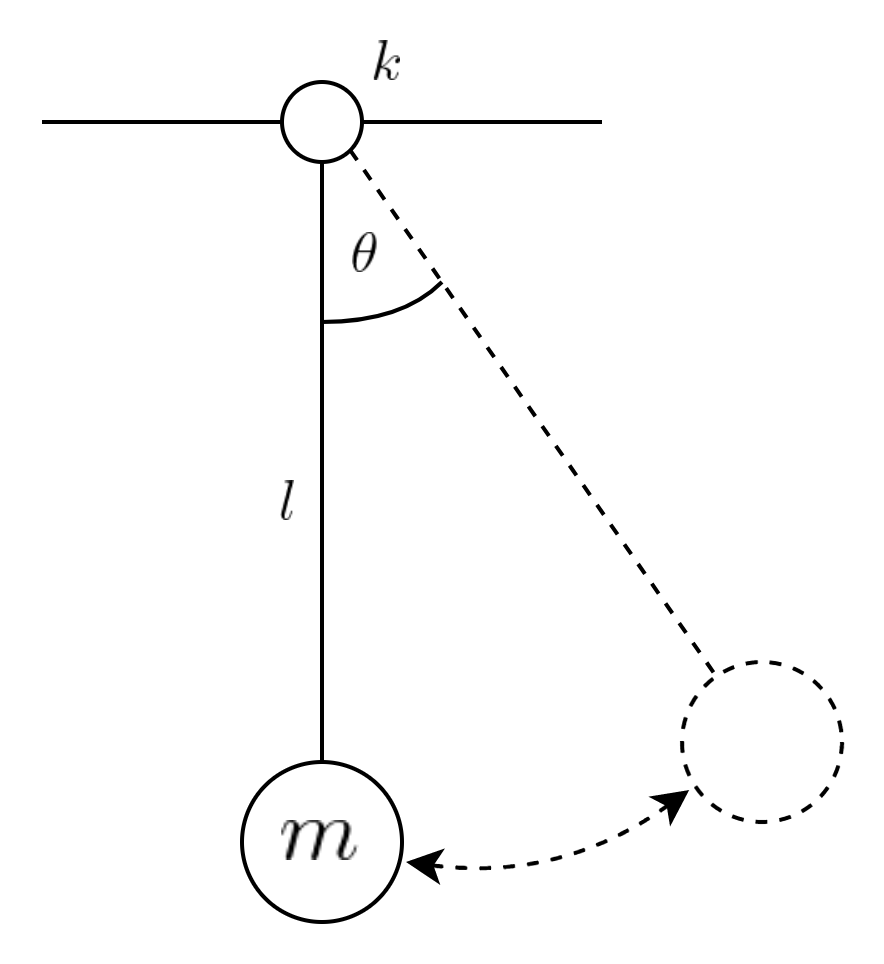
\includegraphics[width = 0.5\textwidth]{assets/image/soal_1.png}
                    \caption{Sistem pendulum}
                    \label{gambar_1}
                \end{figure}
            \begin{center}
            Keterangan :
                \begin{minipage}[c]{8cm}
                    \begin{itemize}
                        \item $\theta$ : sudut gerak pendulum
                        \item $k$ : koefisien gesek pada tumpuan
                        \item $m$ : massa bola pendulum
                        \item $l$ : panjang tali
                    \end{itemize}
                \end{minipage}
            \end{center}
            Sistem dapat dianalisis dengan persamaan sebagai berikut,
            \begin{equation}
                \sum F = ma
                \label{persamaan_1}
            \end{equation}
            Karena sistem merupakan benda putar, maka dilakukan analisis dengan perhitungan torsi dan inersia sistem sebagai berikut,
            \begin{equation}
                \tau_{\text{input}} - \tau_{\text{gerak pendulum}} - \tau_{\text{gesek}} =  ml\alpha
                \label{persamaan_2}
            \end{equation}
            \begin{equation}
                \begin{split}
                    0 - mg\sin{\theta} - kl\dot{\theta} &= ml\ddot{\theta} \\[5pt]
                    -\frac{mg}{ml}\sin{\theta} - \frac{kl}{ml}\dot{\theta} &= \ddot{\theta} \\[5pt]
                    -\frac{g}{l}\sin{\theta} - \frac{k}{m}\dot{\theta} &= \ddot{\theta}
                    \label{persamaan_3}
                \end{split}
            \end{equation}
            dari persamaan diatas didapatkan aturan sebagai berikut,
            \begin{equation}
                \begin{split}
                    x_1 &= \theta \\[5pt]
                    x_2 &= \dot{x_1} = \dot{\theta}
                    \label{persamaan_4}
                \end{split}
            \end{equation}
            Berdasarkan persamaan \eqref{persamaan_3} dan aturan \eqref{persamaan_4} maka dapat disusun persamaan \textit{state space} sebagai berikut,
            \begin{equation}
                \begin{split}
                    \dot{x} &= Ax+Bu \\[5pt]
                    \begin{bmatrix} \dot{x_1} \\ \dot{x_2} \end{bmatrix} &= \begin{bmatrix} 0 & x_2 \\ -\frac{g}{l}\sin{x_1} & -\frac{k}{m}x_2 \end{bmatrix} + \begin{bmatrix} 0 \\ 0 \end{bmatrix} u
                    \label{persamaan_5}
                \end{split}
            \end{equation}
            Berdasarkan analisis pada persamaan \eqref{persamaan_5} diperoleh matriks output sebagai berikut,
            \begin{equation}
                \begin{split}
                    y &= Cx + Du \\[5pt]
                    y &= \begin{bmatrix} 1 & 0 \end{bmatrix} \begin{bmatrix} x_1 \\ x_2 \end{bmatrix}
                    \label{persamaan_6}
                \end{split}
            \end{equation}
        \subsubsection{Simulasi sistem dengan MATLAB}
            Simulasi persamaan sistem dilakukan dengan MATLAB (m-file) kode program untuk simulasi ditunjukkan sebagai berikut,
            \newline
            \lstinputlisting[language = Matlab, style = custom]{assets/code/kode_simulasi_pendulum.m}
            Hasil simulasi pada MATLAB menunjukkan hasil simulasi adalah nol, hal ini terjadi karena pada sistem pendulum tidak ada input yang diberikan sehingga \textit{output} sistem bernilai nol. \textit{output} sistem ditunjukkan pada gambar \ref{gambar_10}
            \begin{figure}[H]
                \centering
                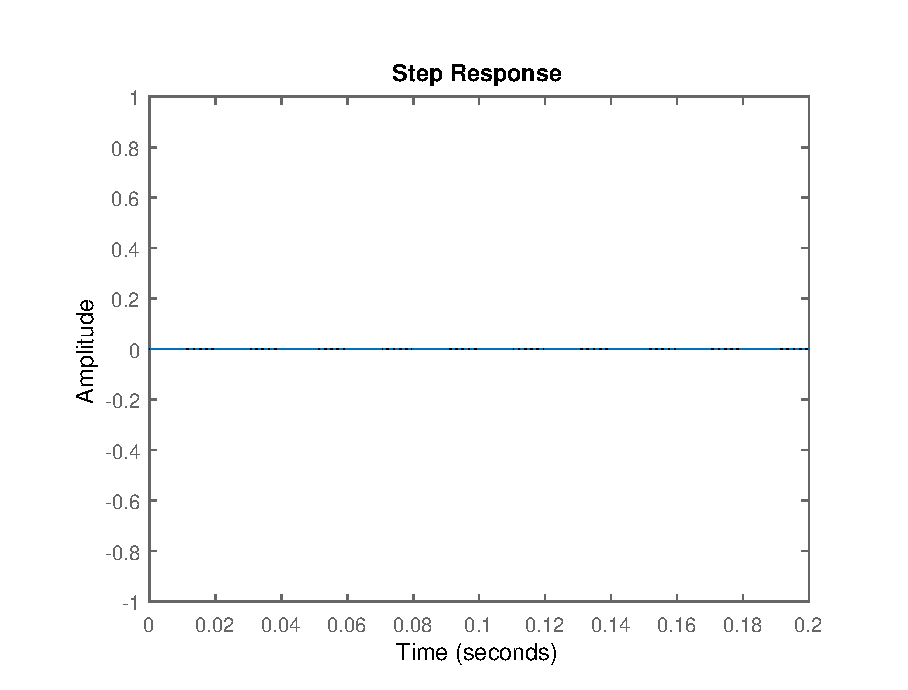
\includegraphics[width = 0.8\textwidth]{assets/image/STATE_SPACE_PENDULUM.eps}
                \caption{Hasil simulasi pemodelan pendulum}
                \label{gambar_10}
            \end{figure}
    \subsection{Pemodelan state space : sistem pendulum terbalik diatas gerobak}
        \subsubsection{Pemodelan matematis sistem}
            Pemodelan sistem pendulum terbalik (\textit{inverted pendulum}) diatas gerobak. sistem digambarkan sebagai berikut,
            \begin{figure}[H]
                \centering
                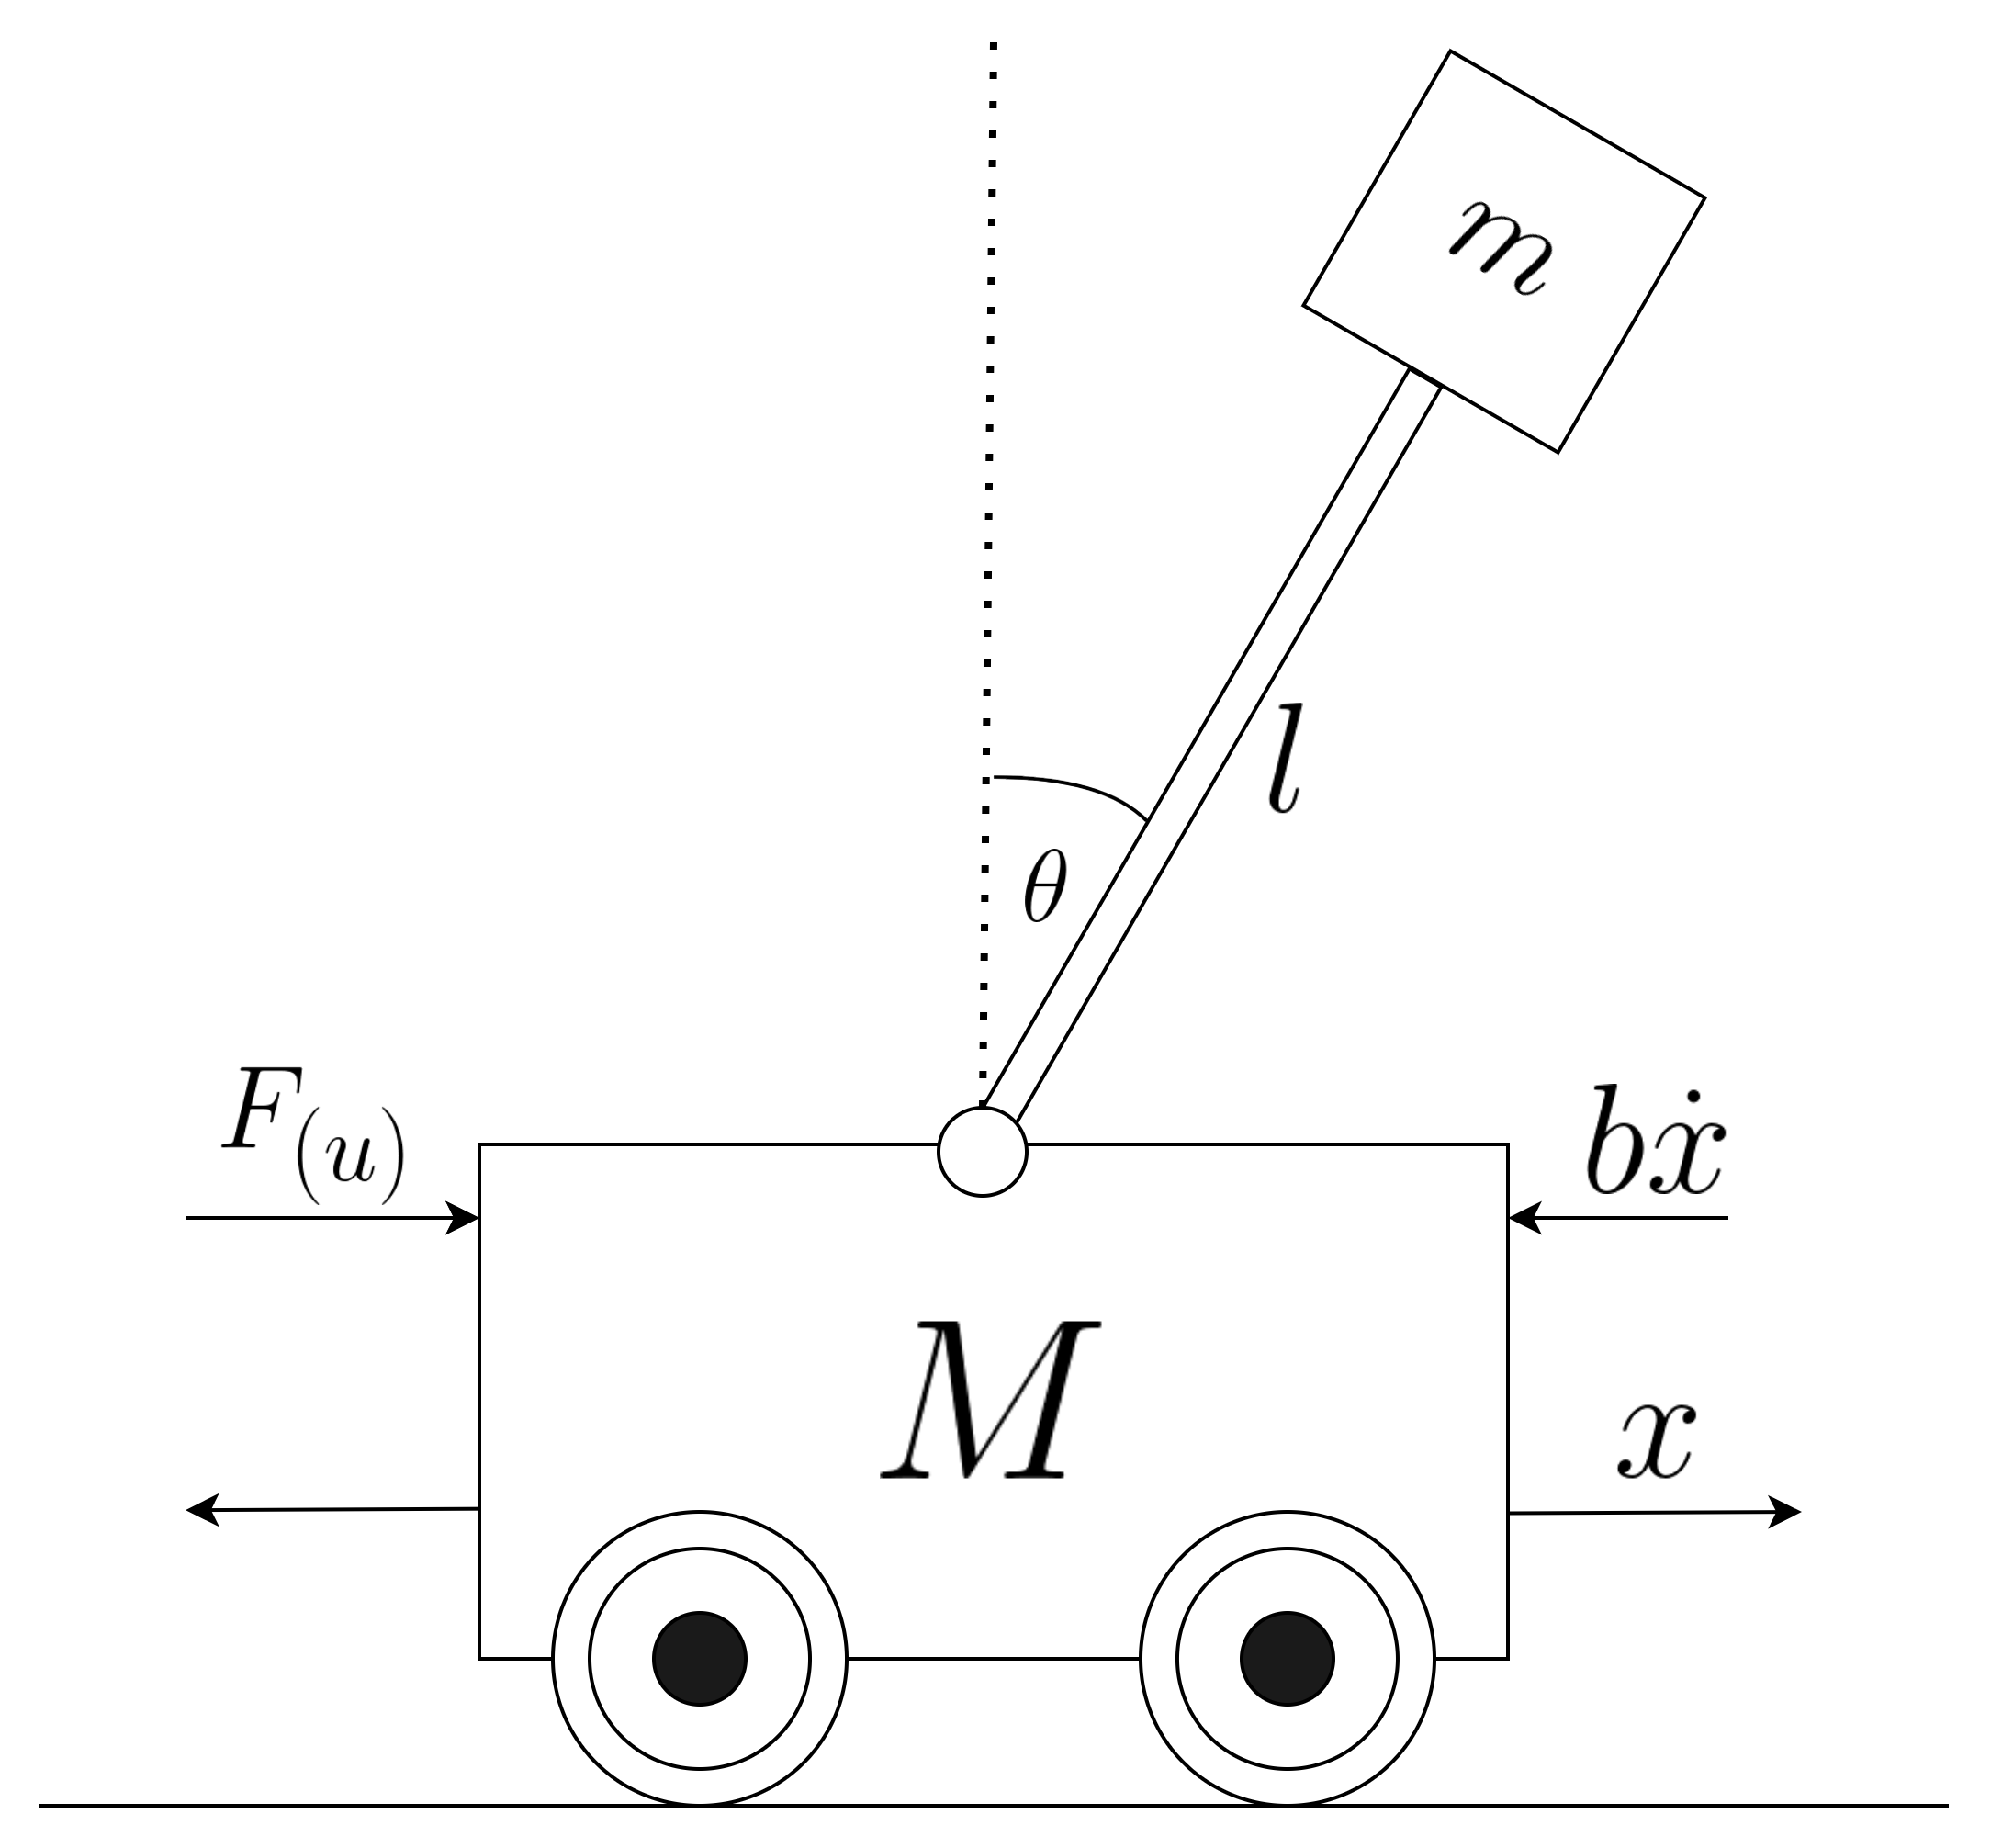
\includegraphics[width = 0.4\textwidth]{assets/image/soal_2.png}
                \caption{Sistem pendulum terbalik diatas gerobak}
                \label{gambar_2}
            \end{figure}
            \begin{center}
            Keterangan :
                \begin{minipage}[c]{8cm}
                    \begin{itemize}
                        \item $\theta$ : sudut ayun pendulum
                        \item $F_{(u)}$ : gaya masukan
                        \item $m$ : massa ujung pendulum
                        \item $M$ : massa gerobak
                        \item $x$ : posisi gerobak terhadap alas
                        \item $b\dot{x}$ : gaya gesek
                    \end{itemize}
                \end{minipage}
            \end{center}
            Pemodelan dan analisa sistem mekanik pendulum terbalik pada gerobak dapat dilakukan menggunakan hukum newton sebagai berikut,
            \begin{equation}
                \sum F = ma
                \label{persamaan_7}
            \end{equation}
            \begin{equation}
                \begin{split}
                    F_{(u)} - F_{gesek} - F_{reaksi} &= ma \\[5pt]
                    F_{(u)} - b\dot{x} - N &= M\ddot{x} \\[5pt]
                    M\ddot{x} + b\dot{x} + N &= F{(u)}
                    \label{persamaan_8}
                \end{split}
            \end{equation}
            \begin{equation}
                N = m\ddot{x} + ml\ddot{\theta}\cos{\theta} + ml\dot{\theta}^2\sin{\theta}
                \label{persamaan_9}
            \end{equation}
            \begin{equation}
                F = (M + m)\ddot{x} + b\dot{x} + ml\ddot{\theta}\cos{\theta} - ml\dot{\theta}^2\sin{\theta}
            \end{equation}
            \begin{equation}
                    P\sin{\theta} + N\cos{\theta} - mg\sin{\theta} = -ml\ddot{x}\cos{\theta}
            \end{equation}
            \begin{equation}
                -Pl\sin{\theta} - Nl\cos{\theta} = I\ddot{\theta}
            \end{equation}
            \begin{equation}
                (I + ml^2)\ddot{\theta} + mgl\sin{\theta} = -ml\ddot{x}\cos{\theta}
            \end{equation}
            \begin{equation}
                \begin{split}
                    \cos{\theta} &= \cos{\pi + \phi} \approx -1 \\[5pt]
                    \sin{\theta} &= \sin{\pi + \phi} \approx -\phi
                \end{split}
            \end{equation}
            \begin{equation}
                \begin{split}
                    (I+ml^2)\ddot{\phi} - mgl\phi = ml\ddot{x} \\[5pt]
                    (M+m)\ddot{x} + b\dot{x} - ml\ddot{\phi} = u \\[10pt]
                \end{split}
            \end{equation}
            \begin{equation*}
                \dot{x} = Ax+Bu \\[5pt]
            \end{equation*}
            \begin{equation}
                \begin{bmatrix} \dot{x} \\ \ddot{x} \\ \dot{\phi} \\ \ddot{\phi} \end{bmatrix} = \begin{bmatrix} 0 & 1 & 0 & 0 \\ 0 & \frac{-(I+ml^2)b}{I(M+m)+Mml^2} & \frac{m^2gl^2}{I(M+m)+Mml^2} & 0 \\ 0 & 0 & 0 & 1 \\ 0 & \frac{-mlb}{I(M+m)+Mml^2} & \frac{mgl(M+m)}{I(M+m)+Mml^2} & 0\end{bmatrix} \begin{bmatrix} x \\ \dot{x} \\ \phi \\ \dot{\phi} \end{bmatrix} + \begin{bmatrix}
                        0 \\ \frac{I + ml^2}{I(M+m)+Mml^2} \\ 0 \\ \frac{ml}{I(M+m)+Mml^2} \end{bmatrix} \\[10pt]
            \end{equation}
            \begin{equation*}
                y = Cx+Du \\[5pt]
            \end{equation*}
            \begin{equation}
                y = \begin{bmatrix} 1 & 0 & 0 & 0 \\ 0 & 0 & 1 & 0 \end{bmatrix} \begin{bmatrix} x\\ \dot{x} \\ \phi \\ \dot{\phi}\end{bmatrix} + \begin{bmatrix}
                    0 \\ 0 \end{bmatrix} u
            \end{equation}
        \subsubsection{Simulasi sistem dengan MATLAB}
            Simulasi sistem dilakukan menggunakan MATLAB dengan kode program berikut,
            \newline
            \lstinputlisting[language = Matlab, style = custom]{assets/code/kode_simulasi_inverted_pendulum.m}
            Dari respon sistem yang ditunjukkan pada gambar \ref{gambar_11} dapat dilihat bahwa sistem memberikan respon ketika diberikan gaya input.
            \begin{figure}[H]
                \centering
                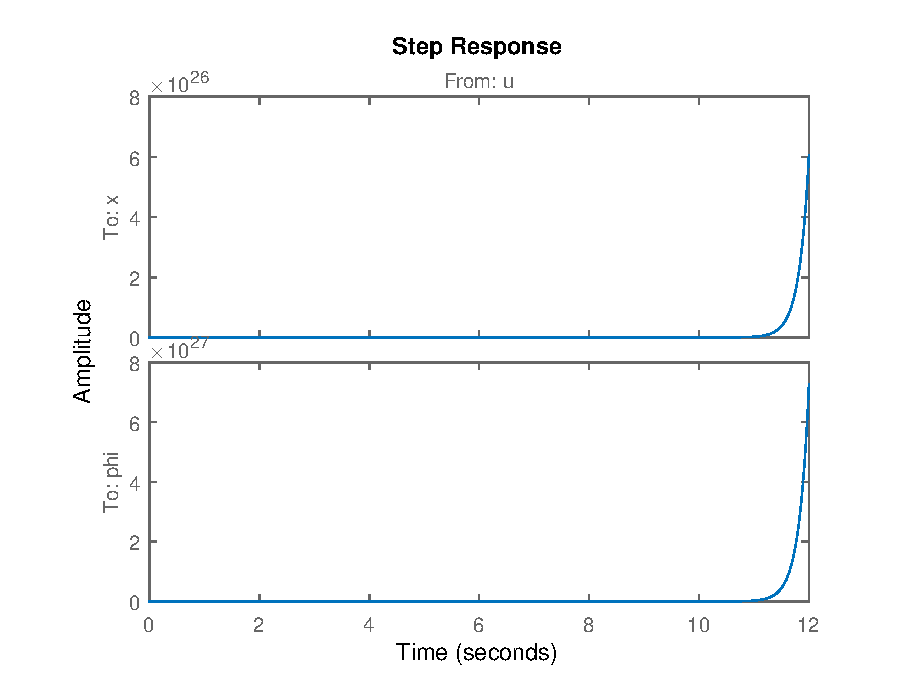
\includegraphics[width = 0.8\textwidth]{assets/image/STATE_SPACE_INVERTED_PENDULUM.eps}
                \caption{Hasil simulasi sistem dengan MATLAB}
                \label{gambar_11}
            \end{figure}
    \subsection{Pemodelan motor DC ke fungsi alih dan state space}
        Pemodelan sistem motor DC dapat dilakukan dengan mencari fungsi mekanik dan elektrik dari sistem tersebut. model sistem motor DC dapat dilihat pada gambar berikut,
        \begin{figure}[H]
            \centering
            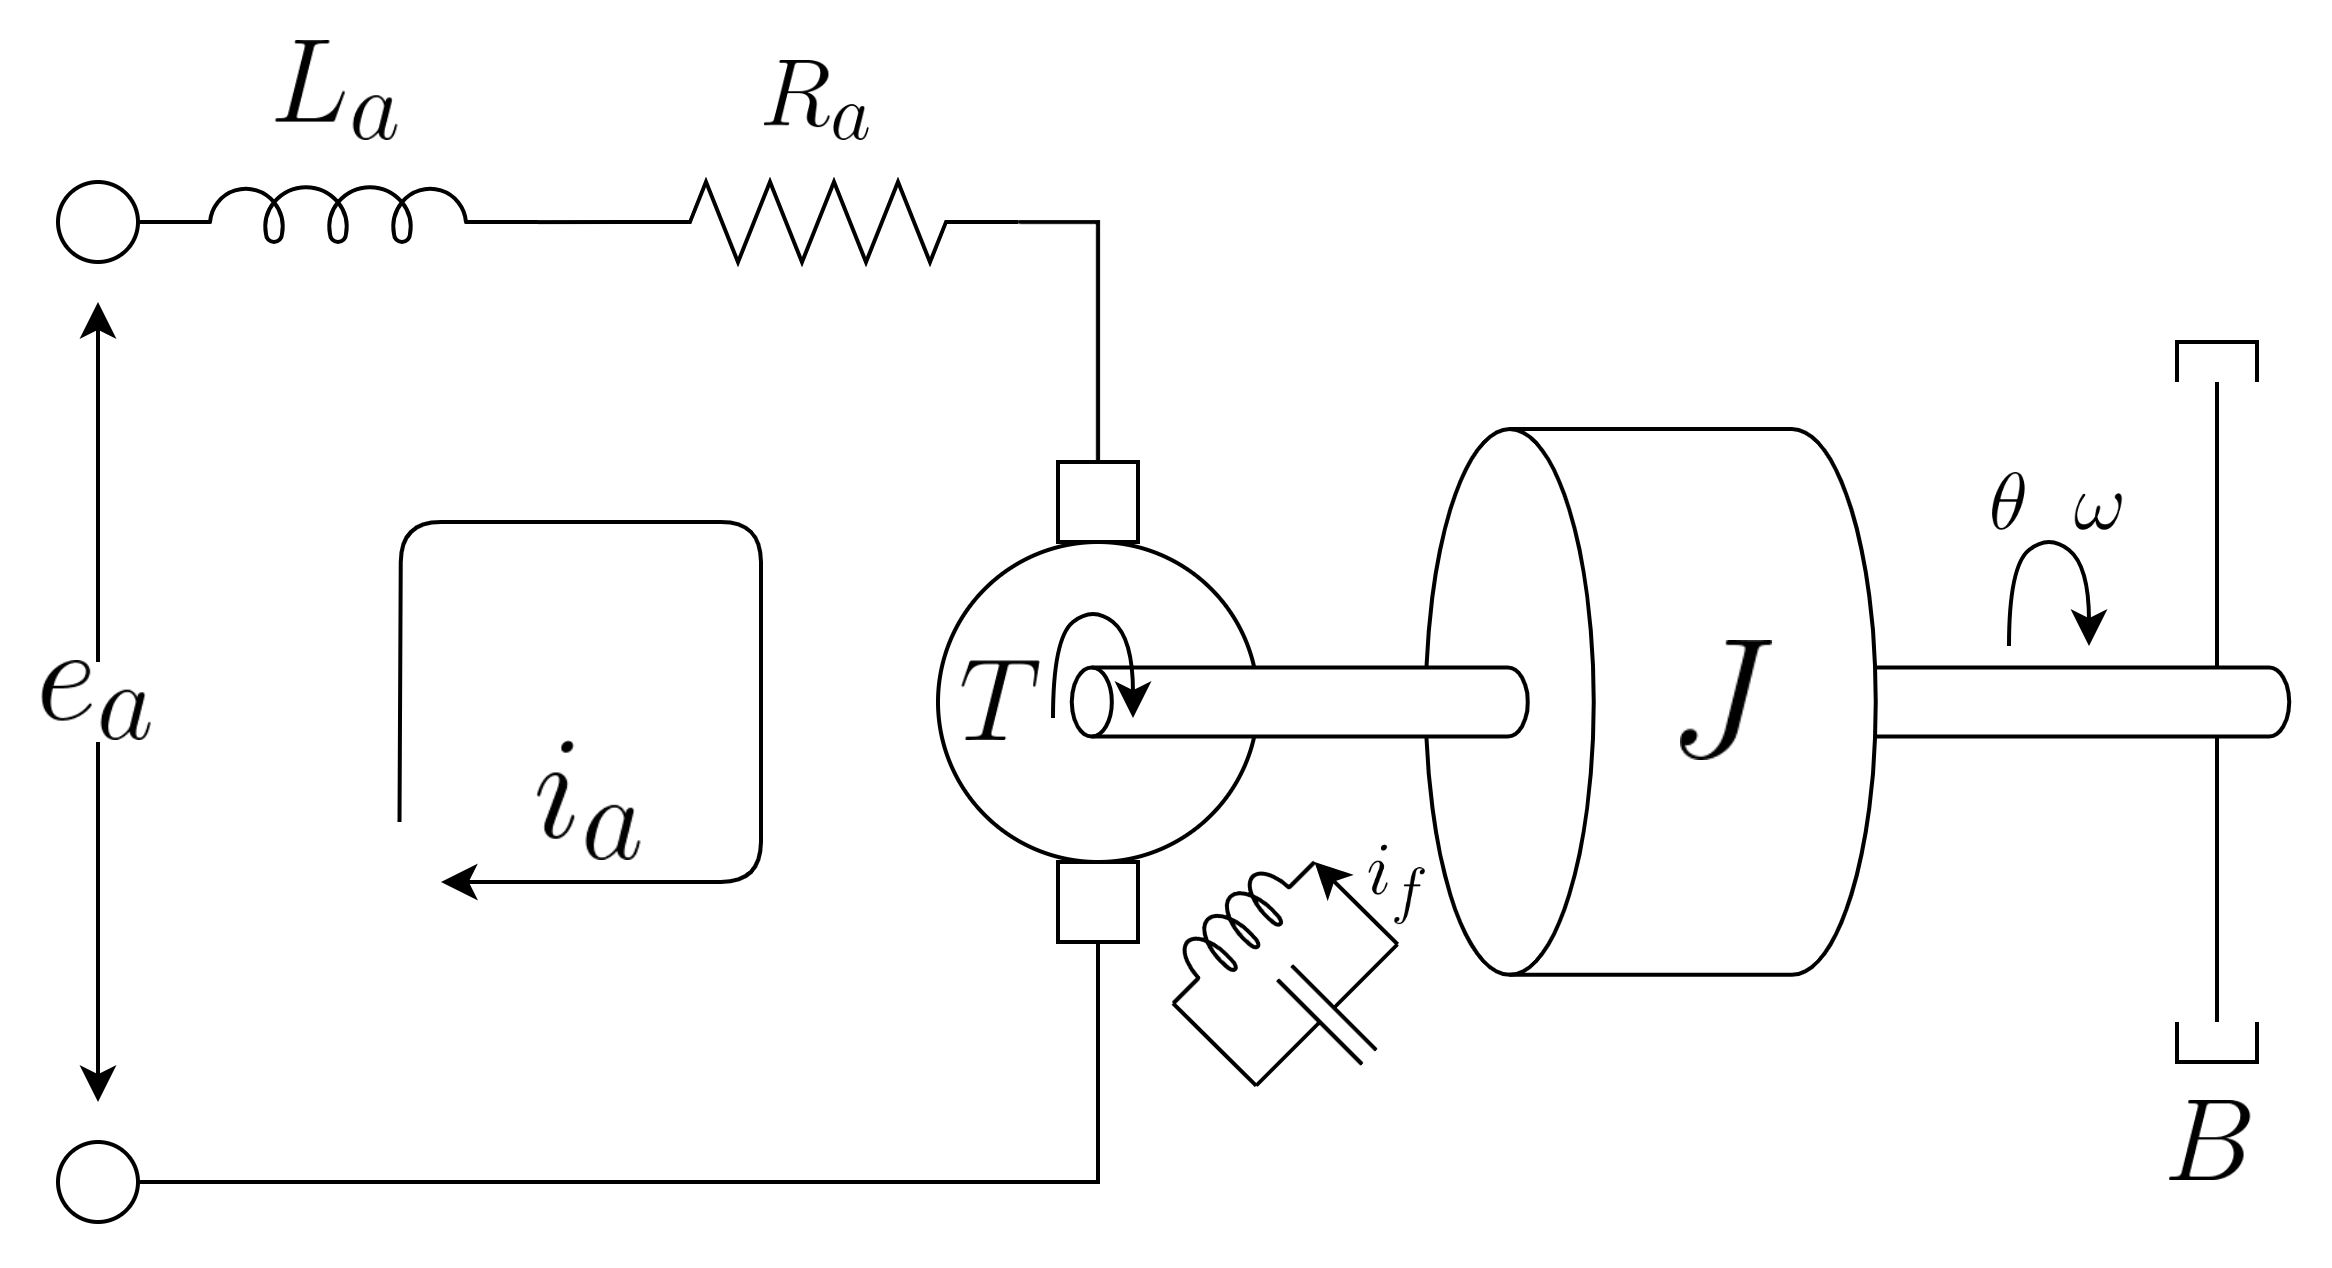
\includegraphics[width = 0.6\textwidth]{assets/image/pemodelan_motor.png}
            \caption{Pemodelan elektrik dan mekanik dari motor DC}
            \label{gambar_3}
        \end{figure}
        \begin{center}
        Keterangan :
            \begin{minipage}[c]{8cm}
                \begin{itemize}
                    \item $\theta$ : posisi motor
                    \item $\omega$ : kecepatan motor
                    \item $T$      : torsi
                    \item $L_a$    : induktansi motor
                    \item $R_a$    : resistansi motor
                    \item $J$      : momen inersia
                    \item $B$      : gesekan viskos
                \end{itemize}
            \end{minipage}
        \end{center}
        \subsubsection{Persamaan rangkaian elektrik motor DC}
            \begin{figure}[H]
                \centering
                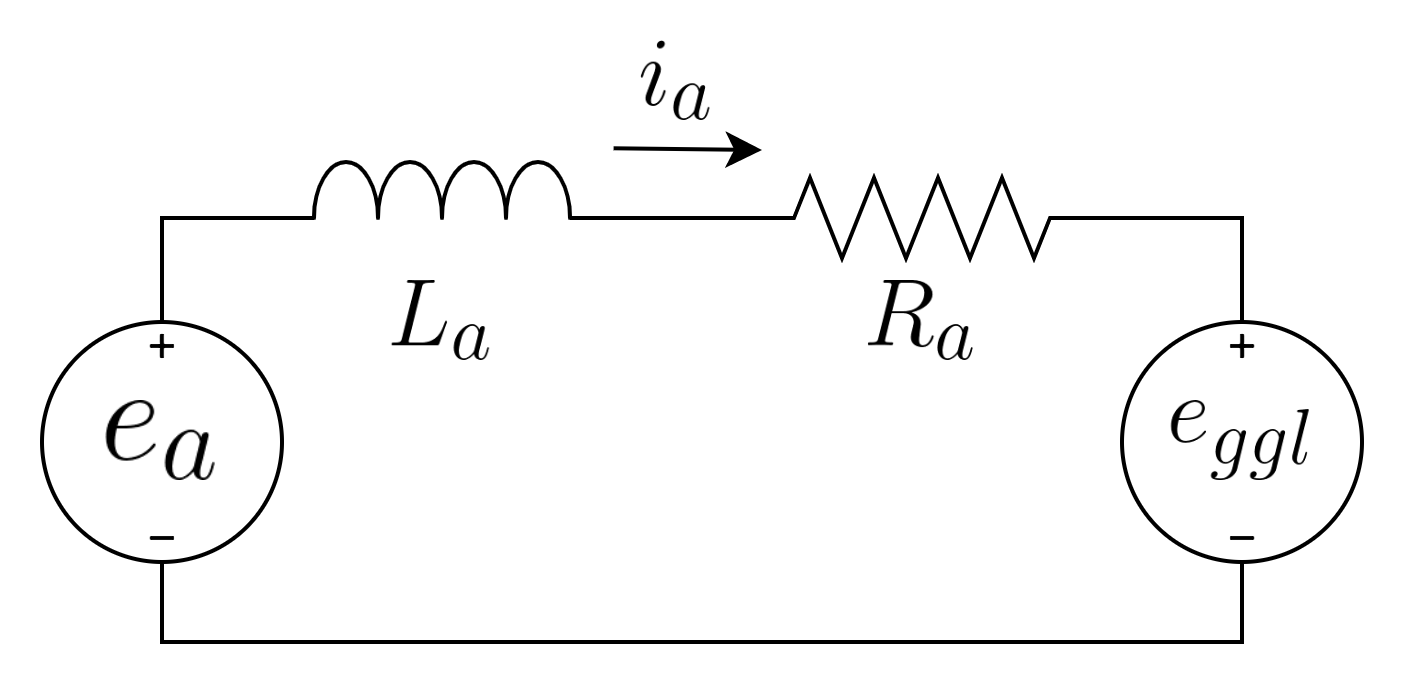
\includegraphics[width = 0.5\textwidth]{assets/image/pemodelan_sirkuit_motor.png}
                \caption{Pemodelan sirkuit dari motor DC}
                \label{gambar_4}
            \end{figure}
            Persamaan rangkaian elektrik pada motor dapat dianalisa dengan hukum kirchoff sebagai berikut,
            \begin{equation}
                \begin{split}
                    e_a - e_{ggl} &= L_a \frac{di_a}{dt} + R_a i_a \\[5pt]
                    e_a &= L_a \frac{di_a}{dt} + R_a i_a + e_{ggl}
                    \label{persamaan_10}
                \end{split}
            \end{equation}
        \subsubsection{Persamaan tegangan gaya gerak listrik pada motor DC}
        \textit{back emf} atau tegangan balik dapat diperoleh dengan mengalikan konstanta motor dengan kecepatan sudut motor. Arus medan ($i_f$) bernilai konstan sehingga nilai arus medan tidak disertakan dalam analisa.
            \begin{equation}
                \begin{split}
                    e_{ggl} &= K_m i_f \frac{d\theta}{dt} \\[5pt]
                    e_{ggl} &= K_m \frac{d\theta}{dt}
                    \label{persamaan_11}
                \end{split}
            \end{equation}
        \subsubsection{Persamaan elektrik motor DC}
            Dari persamaan \eqref{persamaan_10} dan persamaan \eqref{persamaan_11} didapatkan persamaan state $\dot{i_a}$ sebagai berikut,
            \begin{equation}
                \begin{split}
                    e_a &= L_a\frac{di_a}{dt} + R_a i_a + K_m\frac{d\theta}{dt} \\[5pt]
                    L_a\frac{di_a}{dt} &= -K_m\frac{d\theta}{dt} - R_a i_a + e_a \\[5pt]
                    \frac{di_a}{dt} &= -\frac{K_m}{L_a}\frac{d\theta}{dt} - \frac{R_a}{L_a}i_a + \frac{1}{L_a}e_a \\[5pt]
                    \dot{i_a} &= -\frac{K_m}{L_a}\dot{\theta} - \frac{R_a}{L_a}i_a + \frac{1}{L_a}e_a
                    \label{persamaan_12}
                \end{split}
            \end{equation}
        \subsubsection{Persamaan torsi motor DC}
            \begin{figure}[H]
                \centering
                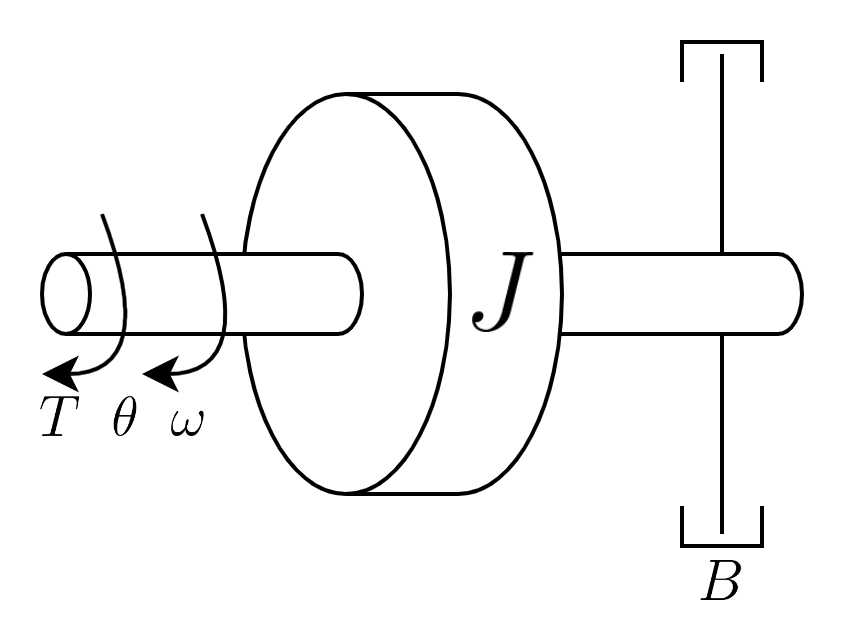
\includegraphics[width = 0.5\textwidth]{assets/image/pemodelan_mekanik_motor.png}
                \caption{Pemodelan mekanik dari motor DC}
                \label{gambar_5}
            \end{figure}
            Hubungan torsi motor terhadap inertia dan gesekan viskos dapat dianalisa dengan persamaan berikut,
            \begin{equation}
                \begin{split}
                    \sum T &= J\alpha \\[5pt]
                    T - B\frac{d\theta}{dt} &= J\frac{d^2\theta}{dt^2} \\[5pt]
                    T &= J\frac{d^2\theta}{dt^2} + B\frac{d\theta}{dt}
                    \label{persamaan_13}
                \end{split}
            \end{equation}
            Hubungan torsi motor dengan arus kumparan jangkar dan flux magnetik dianalisa dengan persamaan berikut,
            \begin{equation}
                \begin{split}
                    B &= \frac{\mu_f n_f i_f}{2\pi l_f} \\[5pt]
                    B &= K_B i_f \\[5pt]
                    \label{persamaan_14}
                \end{split}
            \end{equation}
            \begin{equation}
                \begin{split}
                    T &= K_B i_f i_a l_a r_a n_a \\[5pt]
                    T &= K_{TM} i_f i_a \\[5pt]
                    T &= K_{TM} i_a
                    \label{persamaan_15}
                \end{split}
            \end{equation}
            Dari persamaan torsi \eqref{persamaan_13} dan persamaan torsi \eqref{persamaan_15} dapat diperoleh persamaan \textit{state} $\ddot{\theta}$ sebagai berikut,
            \begin{equation}
                \begin{split}
                    J\frac{d^2\theta}{dt^2} + B\frac{d\theta}{dt} &= K_{TM} i_a \\[5pt]
                    -B \frac{d\theta}{dt} + K_{TM}i_a &= J\frac{d^2\theta}{dt^2} \\[5pt]
                    -\frac{B}{J}\frac{d\theta}{dt} + \frac{K_{TM}}{J}i_a &= \frac{d^2\theta}{dt^2} \\[5pt]
                    -\frac{B}{J}\dot{\theta} + \frac{K_{TM}}{J}i_a &= \ddot{\theta}
                    \label{persamaan_16}
                \end{split}
            \end{equation}
        \subsubsection{Model state space motor DC}
            dari persamaan \eqref{persamaan_12} dan persamaan \eqref{persamaan_16} dapat diperoleh persamaan state space dengan aturan sebagai berikut,
            \begin{equation}
                \begin{split}
                    x_1 &= \dot{\theta} \\[5pt]
                    \dot{x_1} &= \ddot{\theta} \\[5pt]
                    x_2 &= i_a \\[5pt]
                    \dot{x_2} &= \dot{i_a}
                    \label{persamaan_17}
                \end{split}
            \end{equation}
            persamaan \eqref{persamaan_12} dan \eqref{persamaan_16} didefinisikan sesuai dengan peraturan \eqref{persamaan_17} sebagai berikut,
            \begin{equation}
                \dot{x_2} = -\frac{K_m}{L_a}x_1 - \frac{R_a}{L_a}x_2 + \frac{1}{L_a}e_a
                \label{persamaan_18}
            \end{equation}
            \begin{equation}
                \dot{x_1} = -\frac{B}{J}x_1 + \frac{K_{TM}}{J}x_2
                \label{persamaan_19}
            \end{equation}
            Persamaan \eqref{persamaan_18} dan persamaan \eqref{persamaan_19} dapat direpresentasikan dalam bentuk model state space sebagai berikut\cite{Pal},
            \begin{equation}
                \begin{split}
                    \dot{x} &= Ax + Bu \\[5pt]
                    \begin{bmatrix} \dot{x_1} \\ \dot{x_2} \end{bmatrix} &= \begin{bmatrix} -\frac{B}{J} & \frac{K_{TM}}{J} \\ -\frac{K_m}{L_a} & -\frac{R_a}{L_a} \end{bmatrix} \begin{bmatrix}
                        x_1 \\ x_2 \end{bmatrix} + \begin{bmatrix}
                        0 \\ \frac{1}{L_a}\end{bmatrix}e_a
                \end{split}
            \end{equation}
            dihasilkan persamaan \textit{output} state space sebagai berikut,
            \begin{equation}
                \begin{split}
                    y = Cx + Du \\[5pt]
                    y = \begin{bmatrix} 1 & 0 \end{bmatrix} \begin{bmatrix} x_1 \\ x_2 \end{bmatrix}
                \end{split}
            \end{equation}
        \subsubsection{Model fungsi alih laplace motor DC}
            model fungsi alih laplace dari motor DC didapat dari konversi persamaan mekanik (persamaan \eqref{persamaan_15},\eqref{persamaan_16}) dan elektrik (persamaan \eqref{persamaan_10},\eqref{persamaan_11})motor DC ke bentuk laplace sebagai berikut,
            \begin{equation}
                \begin{split}
                    e_a &= L_a \frac{di_a}{dt} + R_a i_a + e_{ggl} \rightarrow E_a = L_a s I_a + R_a I_a \\[5pt]
                    \frac{E_a}{I_a} &= L_a s + R_a \rightarrow \frac{I_a}{E_a} = \frac{1}{L_a s + R_a}\\[10pt]
                \end{split}
            \end{equation}
            \begin{equation}
                \begin{split}
                    e_{ggl} &= K_m\frac{d\theta}{dt} \rightarrow E_{ggl} = K_m s \Theta \rightarrow \frac{E_{ggl}}{\Theta} = K_m s \\[5pt]
                    e_{ggl} &= K_m\omega \rightarrow E_{ggl} = K_m\Omega \rightarrow \frac{E_{ggl}}{\Omega} = K_m \\[10pt]
                \end{split}
            \end{equation}
            \begin{equation}
                \begin{split}
                    T &= J\frac{d^2\theta}{dt^2} + B\frac{d\theta}{dt} \rightarrow T = Js^2\Theta + Bs\Theta \rightarrow \frac{\Theta}{T} = \frac{1}{Js^2 + Bs} \\[5pt]
                    T &= J\frac{d\omega}{dt} + B\omega \rightarrow T = Js\Omega + B\Omega \rightarrow \frac{\Omega}{T} = \frac{1}{Js + B} \\[10pt]
                \end{split}
            \end{equation}
            \begin{equation}
                T = K_{TM}i_a \rightarrow T = K_{TM}I_a \rightarrow \frac{T}{I_a} = K_{TM} \\[5pt]
            \end{equation}
            Hasil transformasi laplace dari persamaan-persamaan diatas kemudian disusun dalam diagram blok dan didapatkan diagram blok fungsi alih laplace dari motor DC sebagai berikut\cite{Arifin},
            \begin{figure}[H]
                \centering
                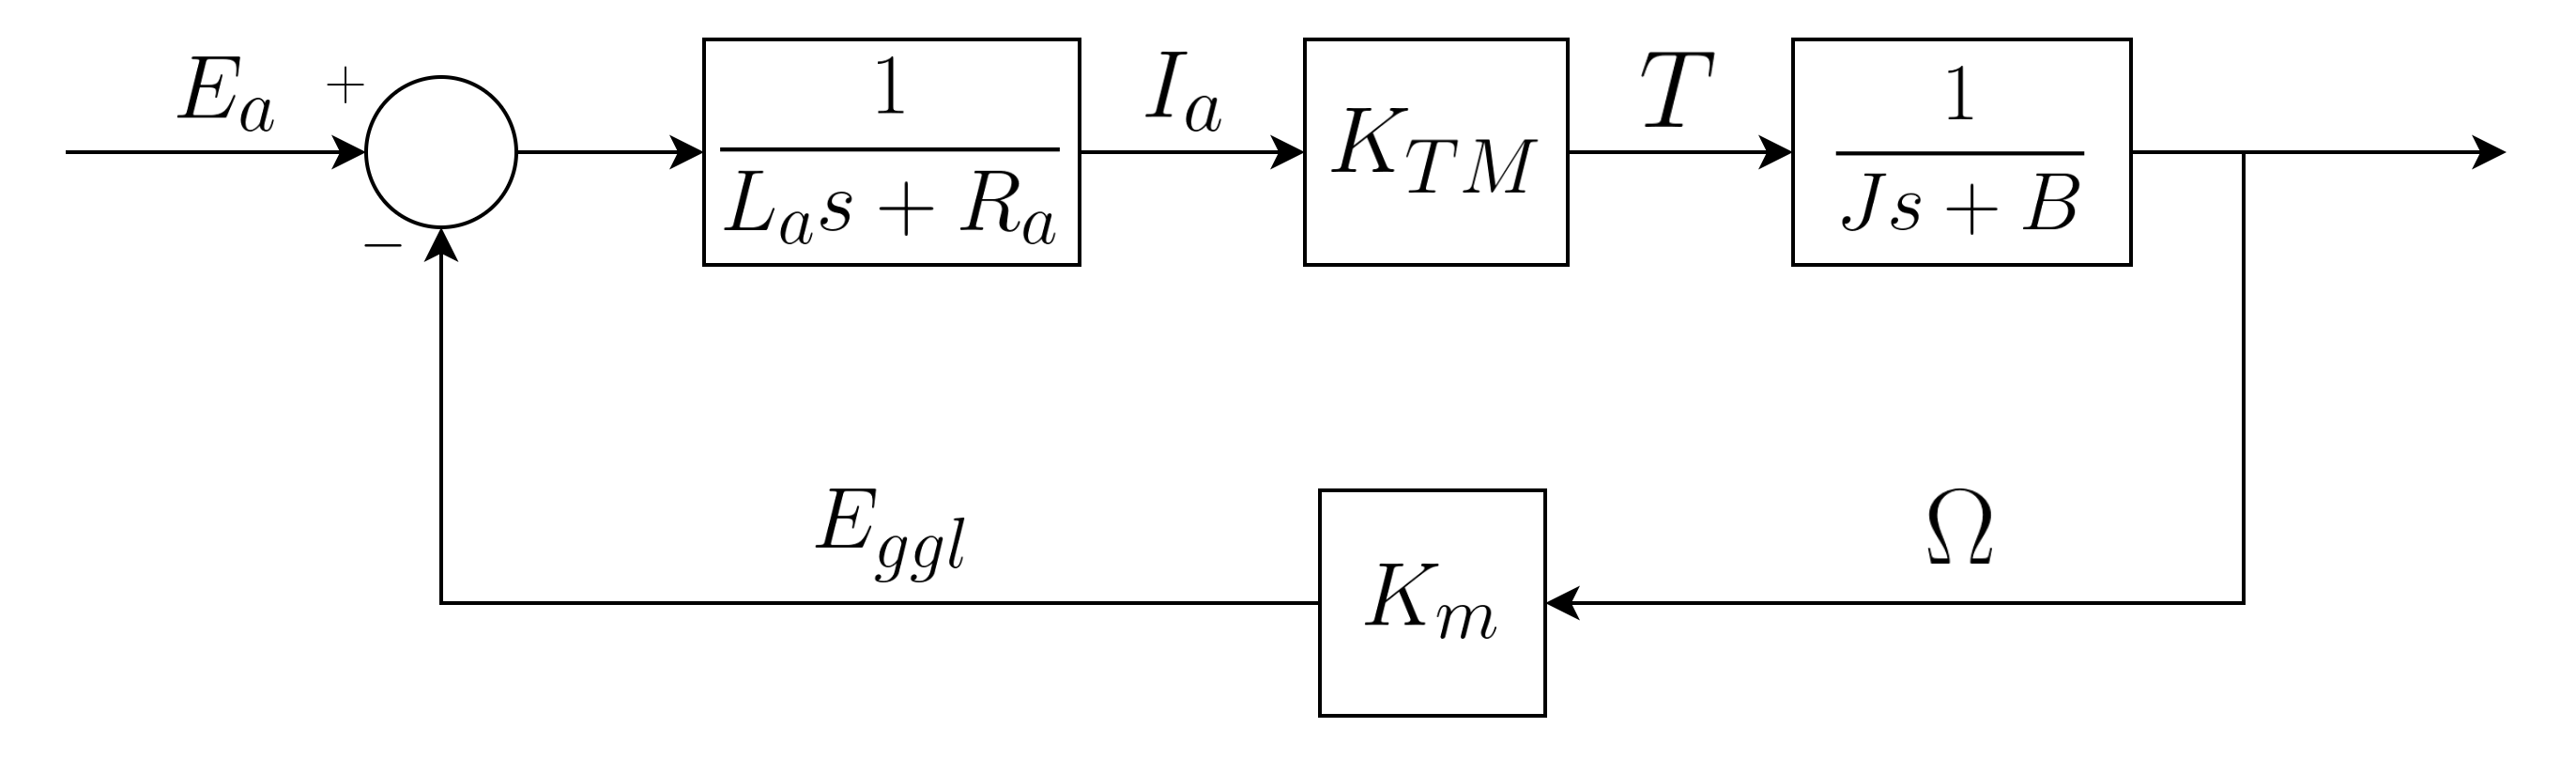
\includegraphics[width = 0.9\textwidth]{assets/image/pemodelan_laplace_motor_dc.png}
                \caption{Diagram blok fungsi alih motor DC (\textit{output} kecepatan)}
                \label{gambar_6}
            \end{figure}
        \subsubsection{Simulasi pemodelan dengan MATLAB}
            diperoleh pemodelan state space dan fungsi alih laplace dari sistem motor DC. Model kemudian disimulasikan menggunakan m-file (model state space) dan Simulink (model laplace). Masing - masing model diberikan fungsi step dengan input tengangan armatur sebesar 12 Volt. Berikut merupakan kode program untuk simulasi pemodelan laplace pada m-file,
            \newline
            \lstinputlisting[language = Matlab]{assets/code/kode_state_space.m}
            Gambar \ref{gambar_7} merupakan hasil plot sistem motor DC dari program m-file yang telah dijalankan, terlihat sistem stabil dan tidak mengalami \textit{overshoot} maupun osilasi.
            \begin{figure}[H]
                \centering
                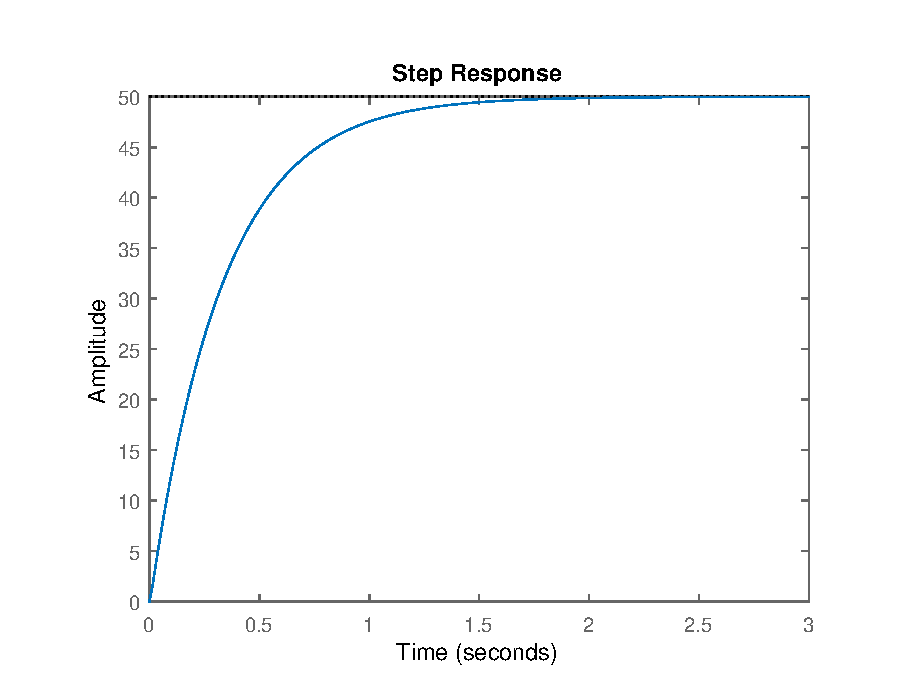
\includegraphics[width = 0.8\textwidth]{assets/image/STATE_SPACE_MOTOR_DC.eps}
                \caption{Hasil step respon model state space motor DC}
                \label{gambar_7}
            \end{figure}
            Gambar \ref{gambar_8} merupakan diagram blok sistem fungsi alih laplace motor DC. Nilai-nilai parameter yang digunakan pada pemodelan laplace dan pemodelan state space adalah sama. 
            \begin{figure}[H]
                \centering
                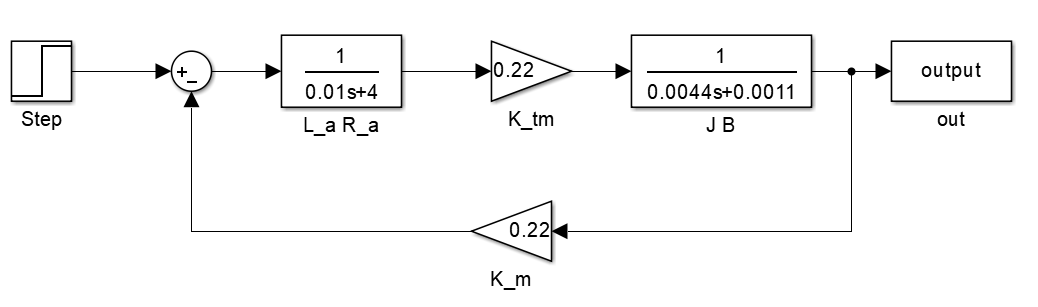
\includegraphics[width = 0.8\textwidth]{assets/image/SIMULINK.png}
                \caption{Diagram blok simulasi transfer function motor DC}
                \label{gambar_8}
            \end{figure}
            Hasil simulasi pada gambar \ref{gambar_9} menunjukkkan bahwa sistem hasil pemodelan fungsi alih dengan sistem pemodelan laplace memiliki hasil yang sama. Sehingga dapat disimpulkan bahwa pemodelan state space yang telah dilakukan memiliki hasil yang konsisten dengan model fungsi alih laplace.
            \begin{figure}[H]
                \centering
                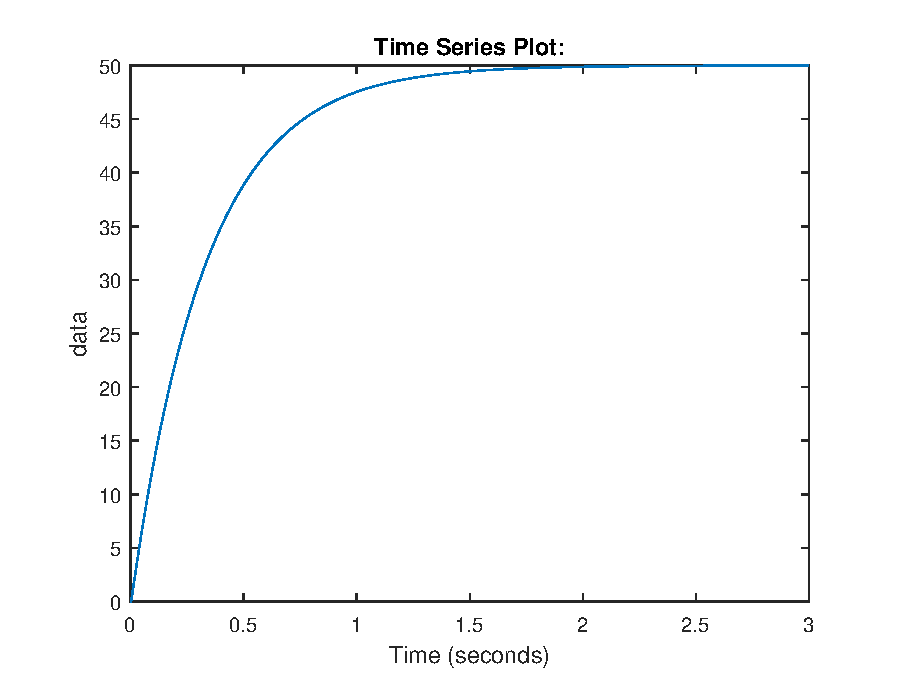
\includegraphics[width = 0.8\textwidth]{assets/image/TRANSFER_FUNCTION_MOTOR_DC.eps}
                \caption{Hasil step respon model transfer function laplace motor DC}
                \label{gambar_9}
            \end{figure}
            
\section{Kesimpulan}
    Pemodelan state space merupakan pemodelan yang dapat digunakan untuk menganalisa sistem mekanik, sistem elektrik, ataupun sistem elektromekanik (seperti motor DC). Pemodelan state space pada sistem dapat dilakukan dengan memodelkan dan menentukan \textit{state} dari sebuah sistem. Hasil pemodelan kemudian digunakan pada persamaan state space $\dot{x} = Ax+Bu$ dan $y = Cx + Du$. Pada pemodelan sistem, agar sebuah sistem dapat dianalisa maka sistem perlu diberikan input. Tanpa adanya input yang diberikan pada sistem, maka sistem tidak akan memberikan \textit{output}, sehingga sistem tidak dapat dianalisa karakteristiknya.
    
\begin{thebibliography}{2}
    \bibitem[1]{Pal} Pal, D. (2016). Modeling, analysis and design of a dc motor based on state space approach. International Journal of Engineering Research \& Technology (IJERT), 5(2), 293-296.
    \bibitem[2]{Arifin} Arifin, Y., \& Amir, A. (2010). Pemodelan dan pengendalian motor DC menggunakan simulasi MATLAB. MEKTEK, 12(2).
\end{thebibliography}
\end{document}